\documentclass[12pt,a4paper]{report}

\usepackage[a4paper,margin=1in,headheight=14pt]{geometry}
\usepackage{graphicx}
\usepackage{amsmath,amssymb}
\usepackage{booktabs}
\usepackage{fancyhdr}
\usepackage{hyperref}
\usepackage{xcolor}
\usepackage{listings}
\usepackage{float}
\usepackage{caption}
\usepackage{subcaption}
\usepackage{titlesec}
\usepackage{enumitem}
\usepackage{tikz}

\hypersetup{
    colorlinks=true,
    linkcolor=blue!60!black,
    urlcolor=blue!60!black,
    citecolor=blue!60!black,
    pdftitle={Wireless Assignment 01 - Hexagonal Cluster Allocation},
    pdfauthor={Suwarna Pyakurel}
}

\definecolor{codebg}{RGB}{248,248,248}
\definecolor{codeframe}{RGB}{180,180,180}
\definecolor{keywordblue}{RGB}{0,0,180}
\definecolor{stringred}{RGB}{163,21,21}
\definecolor{commentgreen}{RGB}{0,128,0}

\lstdefinestyle{pythonstyle}{
    language=Python,
    basicstyle=\ttfamily\small,
    keywordstyle=\color{keywordblue}\bfseries,
    stringstyle=\color{stringred},
    commentstyle=\color{commentgreen}\itshape,
    numbers=left,
    numberstyle=\tiny\color{gray},
    stepnumber=1,
    numbersep=8pt,
    backgroundcolor=\color{codebg},
    frame=single,
    rulecolor=\color{codeframe},
    breaklines=true,
    breakatwhitespace=false,
    showstringspaces=false,
    tabsize=4,
    captionpos=b,
    literate={²}{{$^2$}}1 {√}{{$\sqrt{}$}}1 {×}{{$\times$}}1 {—}{{-}}1 {∠}{{$\angle$}}1 {∴}{{$\therefore$}}1 {°}{{$^\circ$}}1 {✓}{{$\checkmark$}}1 {✗}{{$\times$}}1,
}

\lstset{style=pythonstyle}

\pagestyle{fancy}
\fancyhf{}
\fancyhead[L]{\small Wireless Communication Systems}
\fancyhead[R]{\small Assignment 01}
\fancyfoot[C]{\thepage}
\renewcommand{\headrulewidth}{0.4pt}

\titleformat{\chapter}[display]
{\normalfont\huge\bfseries}{\chaptertitlename\ \thechapter}{12pt}{\Huge}
\titleformat{\section}{\Large\bfseries}{\thesection}{0.8em}{}
\titleformat{\subsection}{\large\bfseries}{\thesubsection}{0.8em}{}

\begin{document}

% ===================== TITLE PAGE =====================
\begin{titlepage}
    \centering
    \vspace*{1.2cm}

    {\Large Institute of Engineering, Purwanchal Campus}\\[0.4cm]
    {\large Department of Electronics, Communication and Information Engineering}\\[1.8cm]

    \rule{\linewidth}{0.8pt}\\[0.6cm]
    {\Huge\bfseries Assignment 01}\\[0.4cm]
    {\LARGE Hexagonal Cellular Cluster Allocation}\\[0.2cm]
    {\large Co-channel Reuse Distance Proof}\\[0.6cm]
    \rule{\linewidth}{0.8pt}\\[2cm]

    {\Large\bfseries Submitted By}\\[0.8cm]
    \begin{tabular}{rl}
        \textbf{Name}      & Suwarna Pyakurel \\[0.25cm]
        \textbf{Roll No.}  & PUR079BEI043 \\[0.25cm]
        \textbf{Email}     & \href{mailto:suwarna.079bei@ioepc.edu.np}{suwarna.079bei@ioepc.edu.np} \\[0.25cm]
        \textbf{Faculty}   & Electronics, Communication and Information Engineering \\[0.25cm]
        \textbf{Level}     & Fourth Year / First Part \\[0.25cm]
        \textbf{Subject}   & Wireless Communication Systems \\
    \end{tabular}

    \vfill
    {\large \today}
\end{titlepage}

\pagenumbering{roman}
\tableofcontents
\clearpage
\pagenumbering{arabic}

% ===================== INTRODUCTION =====================
\chapter{Introduction}

This report presents the complete solution for Assignment 01 in Wireless Communication Systems. The assignment consists of two related tasks:

\begin{enumerate}[label=\arabic*.]
    \item Write a Python program that divides a workspace into regular hexagons and allocates cluster patterns using the formula
    \begin{equation}
        N = i^2 + ij + j^2
    \end{equation}
    where $i$ and $j$ are non-negative integers defining the frequency reuse vector.

    \item Prove that for hexagonal geometry, the co-channel reuse distance is given by
    \begin{equation}
        D = R\sqrt{3N}
    \end{equation}
    where $R$ is the radius of a regular hexagonal cell and $N$ is the cluster size.
\end{enumerate}

The implementation uses \texttt{hexagonal\_cluster.py} for cluster visualization and \texttt{hexagonal\_proof.py} for geometric verification of the reuse distance formula.

% ===================== PART 1: PROGRAM =====================
\chapter{Hexagonal Cluster Allocation Program}

\section{Problem Statement}

Given reuse parameters $i$ and $j$, the program must:
\begin{itemize}
    \item tessellate a workspace into regular hexagonal cells;
    \item compute cluster size $N = i^2 + ij + j^2$;
    \item assign a unique cluster ID to each cell using modular arithmetic on axial coordinates;
    \item display the resulting frequency reuse pattern graphically.
\end{itemize}

\section{Methodology}

\subsection{Coordinate Conversion}

Each cell in the offset grid is converted to axial coordinates $(q, r)$ using the odd-$q$ vertical layout:
\begin{align}
    q &= \text{col} \\
    r &= \text{row} - \frac{\text{col} - (\text{col} \bmod 2)}{2}
\end{align}

\subsection{Cluster Assignment}

The cluster ID for a cell at $(q, r)$ is computed as:
\begin{align}
    c &= \big(q(i+j) - rj\big) \bmod N \\
    d &= (-qj + ri) \bmod N \\
    \text{cluster} &= (c + d) \bmod N
\end{align}

Each cell is labeled with cluster number $(\text{cluster} + 1)$ for display purposes.

\subsection{Hexagon Placement}

For a hexagon of radius $R$, the center of cell $(\text{col}, \text{row})$ is placed at:
\begin{align}
    x &= 1.5 R \cdot \text{col} \\
    y &= \sqrt{3}\, R \left(\text{row} + \tfrac{1}{2}(\text{col} \bmod 2)\right)
\end{align}

\section{Source Code: \texttt{hexagonal\_cluster.py}}

\lstinputlisting[caption={Complete Python implementation for hexagonal cluster allocation.},label={lst:cluster}]{hexagonal_cluster.py}

\section{Program Output}

The program was executed for three representative $(i, j)$ pairs. Each figure shows the cluster number inside every hexagon and uses a distinct color per cluster.

\subsection{Case 1: $i = 1$, $j = 1$, $N = 3$}

\begin{figure}[H]
    \centering
    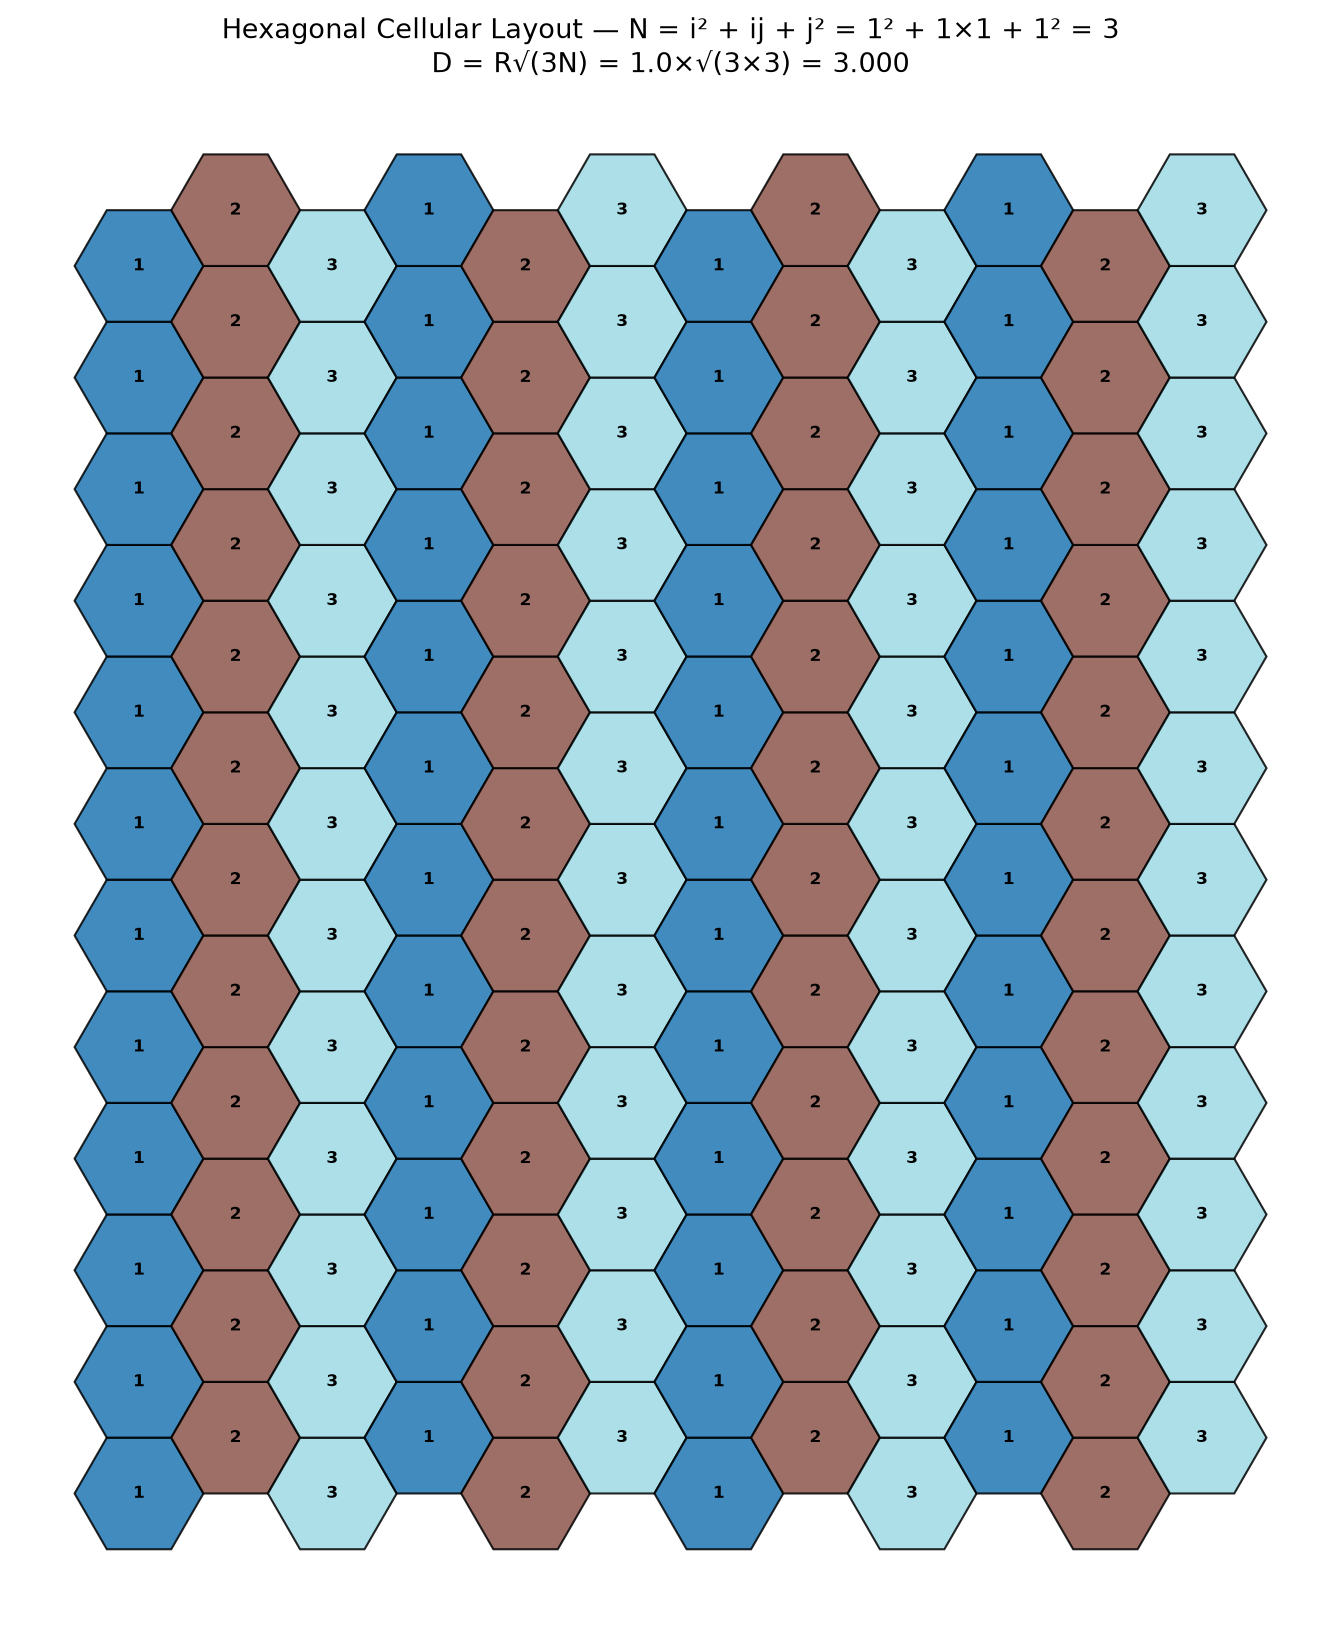
\includegraphics[width=0.82\textwidth]{cluster_1_1.png}
    \caption{Hexagonal layout for $i=1$, $j=1$. Cluster size $N = 1^2 + 1\cdot1 + 1^2 = 3$.}
    \label{fig:cluster11}
\end{figure}

\subsection{Case 2: $i = 2$, $j = 1$, $N = 7$}

\begin{figure}[H]
    \centering
    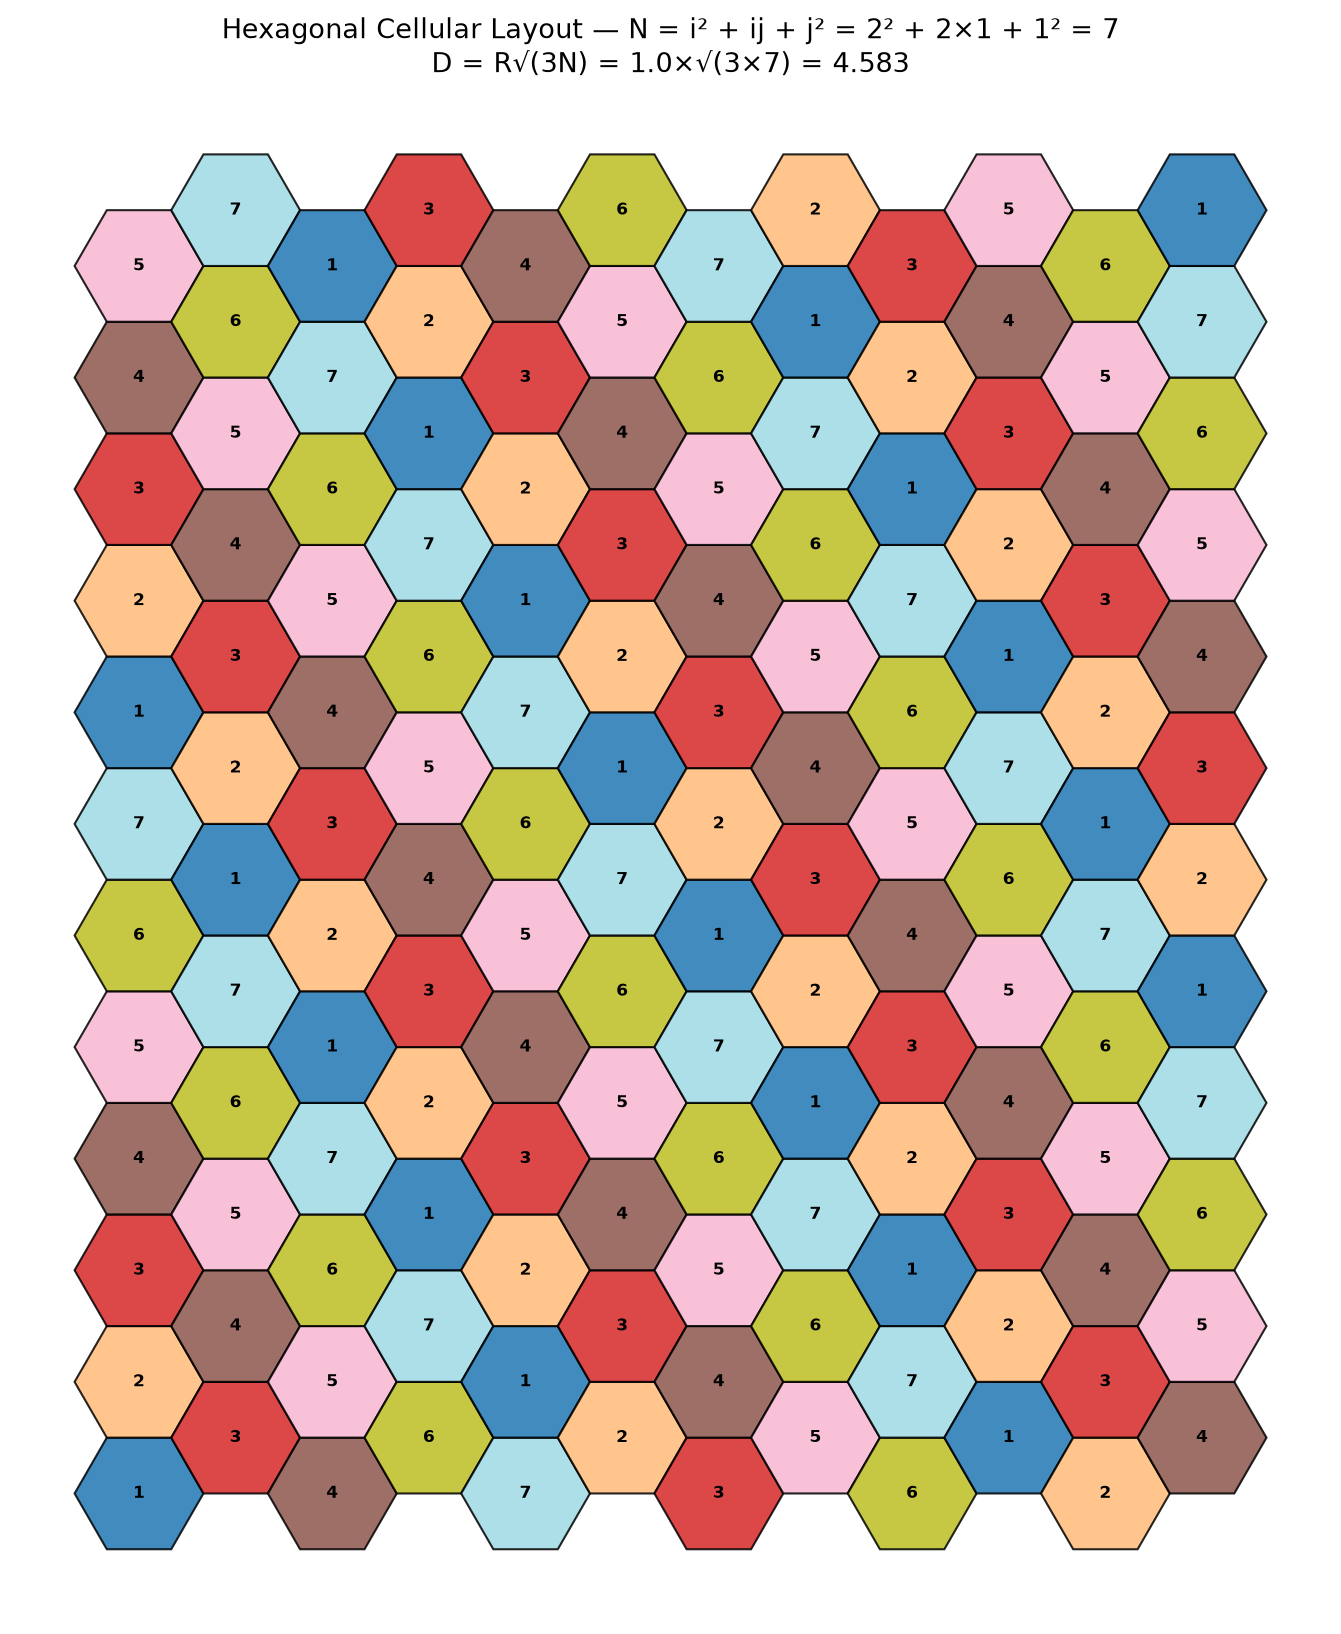
\includegraphics[width=0.82\textwidth]{cluster_2_1.png}
    \caption{Hexagonal layout for $i=2$, $j=1$. Cluster size $N = 2^2 + 2\cdot1 + 1^2 = 7$. Reuse distance $D = R\sqrt{3N} = \sqrt{21} \approx 4.583$.}
    \label{fig:cluster21}
\end{figure}

\subsection{Case 3: $i = 3$, $j = 2$, $N = 19$}

\begin{figure}[H]
    \centering
    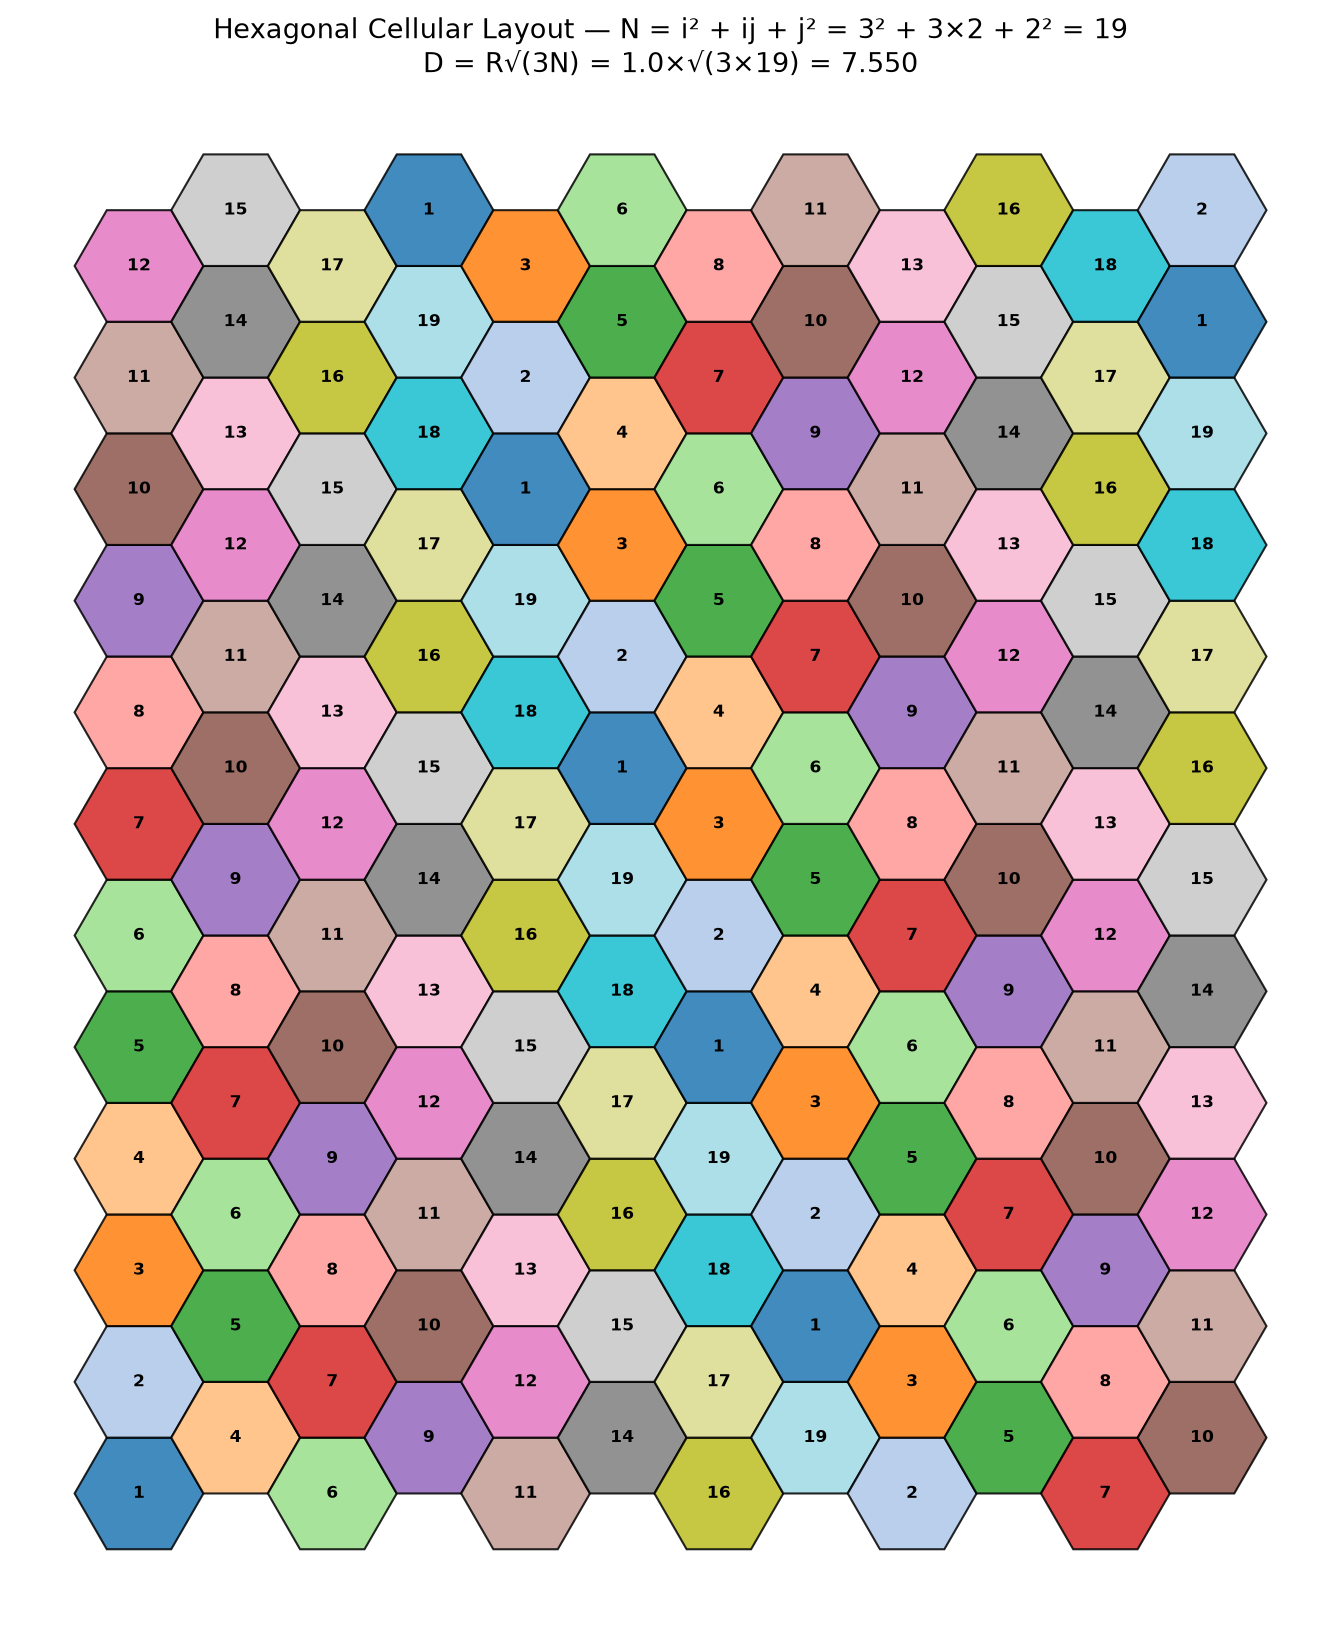
\includegraphics[width=0.82\textwidth]{cluster_3_2.png}
    \caption{Hexagonal layout for $i=3$, $j=2$. Cluster size $N = 3^2 + 3\cdot2 + 2^2 = 19$.}
    \label{fig:cluster32}
\end{figure}

\section{Sample Console Output}

For $i = 2$, $j = 1$, and $R = 1.0$, the program prints:
\begin{verbatim}
Cluster parameters: i = 2, j = 1
Cluster size (N)     = i² + ij + j² = 2² + 2×1 + 1² = 7
Cell radius (R)      = 1.0
Reuse distance (D)   = R√(3N) = 4.5826
Reuse ratio (Q=D/R)  = √(3N) = 4.5826
\end{verbatim}

% ===================== PART 2: PROOF =====================
\chapter{Proof: Co-channel Reuse Distance in Hexagonal Geometry}

\section{Statement}

\textbf{To prove:} For hexagonal cellular geometry,
\begin{equation}
    D = R\sqrt{3N}, \qquad Q = \frac{D}{R} = \sqrt{3N}
\end{equation}
where
\begin{itemize}
    \item $R$ = radius of a regular hexagonal cell (center to vertex),
    \item $N = i^2 + ij + j^2$ = cluster size,
    \item $i, j$ = non-negative integers along two reuse directions,
    \item $D$ = distance between centers of two co-channel cells.
\end{itemize}

\section{Geometric Setup}

Refer to Figure~\ref{fig:proofdiagram}. Starting from co-channel cell center \textbf{A}:
\begin{enumerate}
    \item move $i$ hex steps along adjacent cell centers to reach \textbf{B};
    \item turn through the hex-grid direction and move $j$ steps to reach \textbf{C}.
\end{enumerate}

The co-channel reuse distance is $D = AC$. Let $R_p$ denote half the center-to-center spacing between adjacent cells. Each step has length $2R_p$, so:
\begin{align}
    AB &= i \cdot 2R_p \\
    BC &= j \cdot 2R_p \\
    \angle ABC &= 120^\circ \quad (\cos 120^\circ = -\tfrac{1}{2})
\end{align}

\begin{figure}[H]
    \centering
    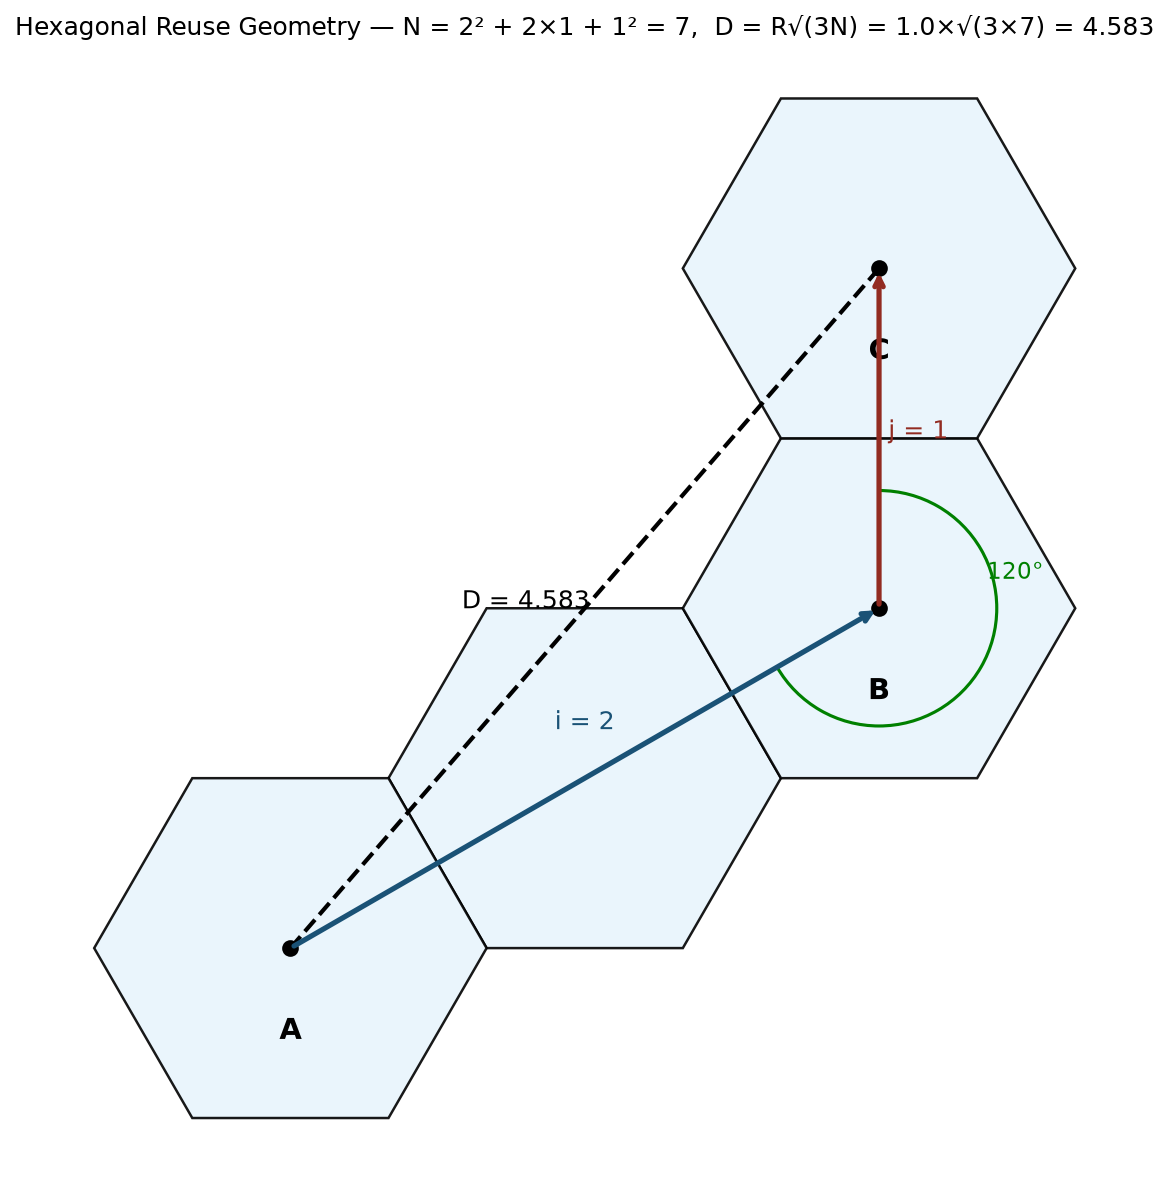
\includegraphics[width=0.78\textwidth]{proof_2_1.png}
    \caption{Reuse geometry for $i=2$, $j=1$. Points A and C are co-channel cell centers separated by distance $D$.}
    \label{fig:proofdiagram}
\end{figure}

\section{Derivation}

\subsection{Step 1: Law of Cosines}

Applying the law of cosines in $\triangle ABC$:
\begin{equation}
    D^2 = (i \cdot 2R_p)^2 + (j \cdot 2R_p)^2 - 2(i \cdot 2R_p)(j \cdot 2R_p)\cos(120^\circ)
\end{equation}

Substituting $\cos(120^\circ) = -\frac{1}{2}$:
\begin{align}
    D^2 &= 4R_p^2 i^2 + 4R_p^2 j^2 - 2 \cdot 4R_p^2 ij \left(-\frac{1}{2}\right) \\
    D^2 &= 4R_p^2 (i^2 + ij + j^2)
    \label{eq:d2}
\end{align}

\subsection{Step 2: Relation Between $R_p$ and $R$}

For a regular hexagon of radius $R$:
\begin{equation}
    R_p = \frac{\sqrt{3}}{2}\, R \qquad \Longrightarrow \qquad 2R_p = \sqrt{3}\, R
\end{equation}

Substituting into \eqref{eq:d2}:
\begin{align}
    D^2 &= 4 \cdot \frac{3R^2}{4} \cdot (i^2 + ij + j^2) \\
    D^2 &= 3R^2 (i^2 + ij + j^2)
\end{align}

\subsection{Step 3: Cluster Size}

By definition of cluster size in hexagonal reuse:
\begin{equation}
    N = i^2 + ij + j^2
\end{equation}

Therefore:
\begin{equation}
    \boxed{D = R\sqrt{3N}}
\end{equation}

The co-channel reuse ratio is:
\begin{equation}
    Q = \frac{D}{R} = \sqrt{3N}
\end{equation}

\section{Numerical Verification ($i = 2$, $j = 1$, $R = 1$)}

\begin{table}[H]
    \centering
    \caption{Numerical verification of the reuse distance formula.}
    \label{tab:verification}
    \begin{tabular}{@{}ll@{}}
        \toprule
        \textbf{Quantity} & \textbf{Value} \\
        \midrule
        $N = i^2 + ij + j^2$ & $2^2 + 2(1) + 1^2 = 7$ \\
        $R_p = \dfrac{\sqrt{3}}{2}R$ & $0.8660$ \\
        $2R_p = \sqrt{3}\,R$ & $1.7321$ \\
        $D$ (law of cosines) & $\sqrt{21} = 4.5826$ \\
        $D = R\sqrt{3N}$ & $\sqrt{3 \times 7} = 4.5826$ \\
        $Q = D/R = \sqrt{3N}$ & $4.5826$ \\
        \bottomrule
    \end{tabular}
\end{table}

Both methods yield identical results, confirming the proof.

\section{Supporting Code: \texttt{hexagonal\_proof.py}}

The proof module verifies the derivation numerically and generates the geometry diagram shown in Figure~\ref{fig:proofdiagram}.

\lstinputlisting[caption={Python module for proof verification and geometry diagram generation.},label={lst:proof}]{hexagonal_proof.py}

% ===================== CONCLUSION =====================
\chapter{Conclusion}

This assignment successfully demonstrates hexagonal frequency reuse in cellular systems. The Python program tessellates a workspace into regular hexagons and assigns cluster IDs using $N = i^2 + ij + j^2$. The mathematical proof establishes that the co-channel reuse distance is $D = R\sqrt{3N}$, which was verified both analytically and numerically for $i = 2$, $j = 1$.

\vspace{1cm}
\begin{center}
    \rule{0.4\textwidth}{0.4pt}\\[0.3cm]
    \textit{--- End of Report ---}
\end{center}

\end{document}
